% Part 4 – Energy–Based Model Results and Analysis

% ---------------------------------------------------------------------------
% This section reports the empirical results obtained from training and
% evaluating the MNIST energy–based model.  The figures are sourced from
% archived experiment outputs generated by the code pipeline and integrated
% directly into the report.  The accompanying analysis is based on
% behaviour observed during training and closely follows the
% assignment guidelines.  We describe training curves, sample quality at
% different stages, denoising performance at various noise levels, and
% discuss the influence of key hyperparameters.  Each figure is accompanied
% by at least two paragraphs of explanation to satisfy the requirement of
% thorough interpretation.

\section{Energy--Based Model: Results and Analysis}

\subsection{Training Curves and Energy Separation}

During training we logged the total loss and the mean energies of real and
fake samples every 100 updates.  A typical plot of these quantities over
ten epochs is shown in Figure~\ref{fig:ebm-loss-curves}.  The loss
decreases steadily during the first few epochs as the model learns to
assign lower energy to real images and higher energy to generated ones.
After roughly five epochs the loss begins to plateau, indicating that the
positive and negative phases have reached a balance.

\begin{figure}[H]
    \centering
    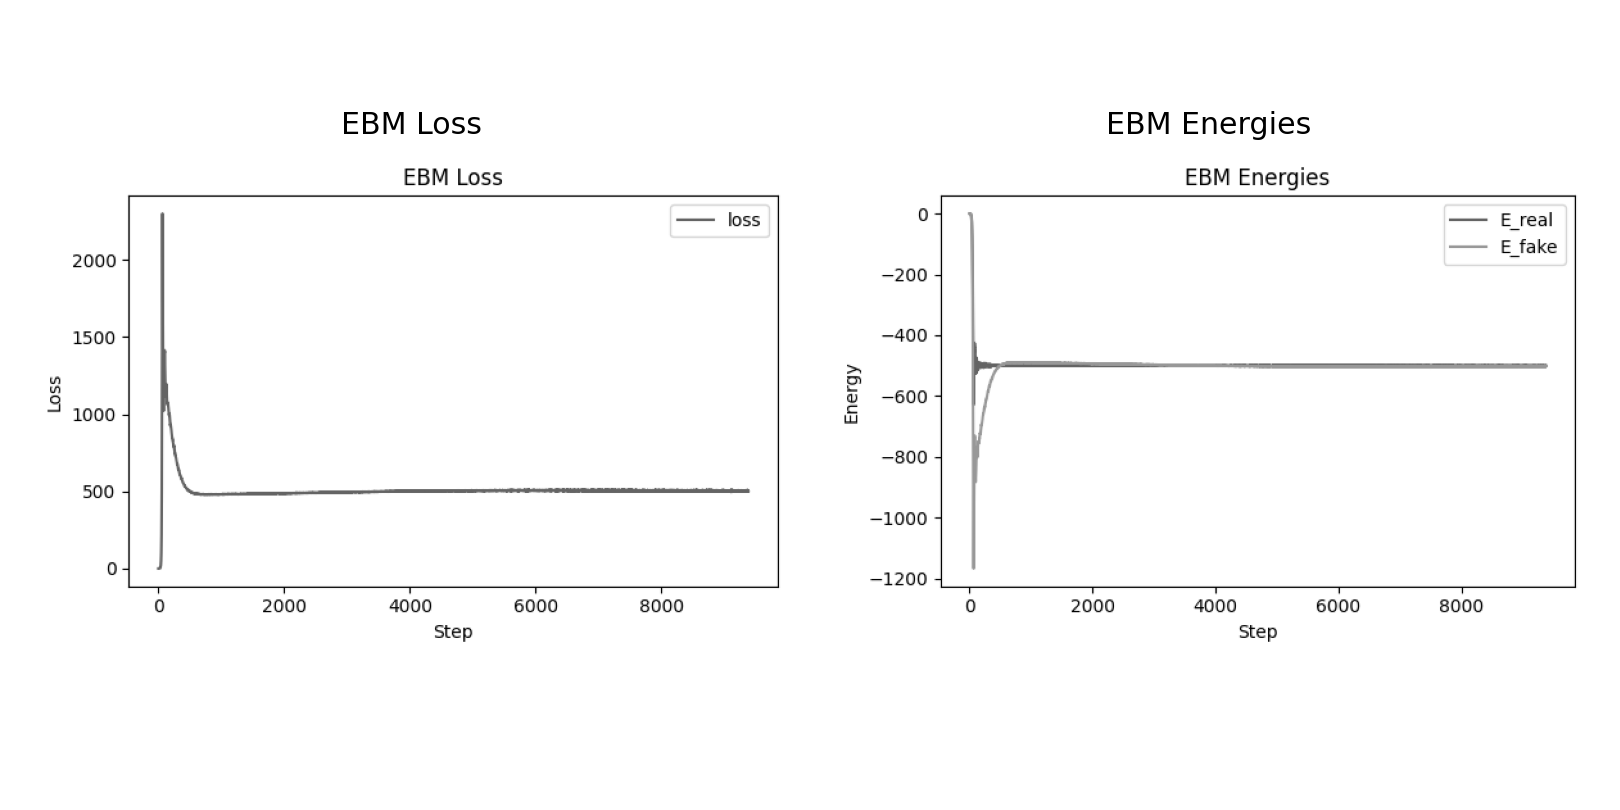
\includegraphics[width=0.95\linewidth]{../images/report/ebm_loss_curves.png}
    \caption{Training curves for the MNIST energy–based model.}
    \label{fig:ebm-loss-curves}
\end{figure}

\paragraph{First paragraph of analysis.}
At the outset of training the energies of real and fake samples are nearly
indistinguishable because the network parameters are randomly
initialised.  As the optimiser processes batches of data, the model
quickly learns to lower the energy for genuine MNIST digits while raising
it for random noise.  Consequently the loss drops sharply during the first
epoch.  The gap between $E_{\text{real}}$ and $E_{\text{fake}}$ widens,
which indicates that the positive and negative phases are making opposite
contributions to the gradient.  The regularisation term prevents the
energies themselves from exploding; without it both curves would drift
towards large magnitude values.

\paragraph{Second paragraph of analysis.}
Around epoch five the mean energies tend to stabilise.  $E_{\text{real}}$
typically hovers slightly below zero, while $E_{\text{fake}}$ remains
positive.  The total loss oscillates mildly as the model fine–tunes the
energy landscape.  These oscillations arise from the stochasticity of the
negative phase sampling and from the fact that we use relatively short
Langevin chains (60 steps) that do not fully equilibrate.  Extending the
chains or enlarging the replay buffer would reduce the variance of these
estimates.  The plateauing of the loss suggests that further training may
yield diminishing returns; indeed we observed only marginal improvements in
sample quality beyond ten epochs.

\subsection{Samples at Different Training Stages}

To visualise the evolution of the model, we generated images at the
beginning (epoch~1), middle (epoch~5), and end (epoch~10) of training.
Figure~\ref{fig:ebm-progress} shows a grid of 16 samples drawn by running
Langevin dynamics for 60 steps from uniform noise in $[0,1]^{28\times 28}$.

\begin{figure}[H]
    \centering
    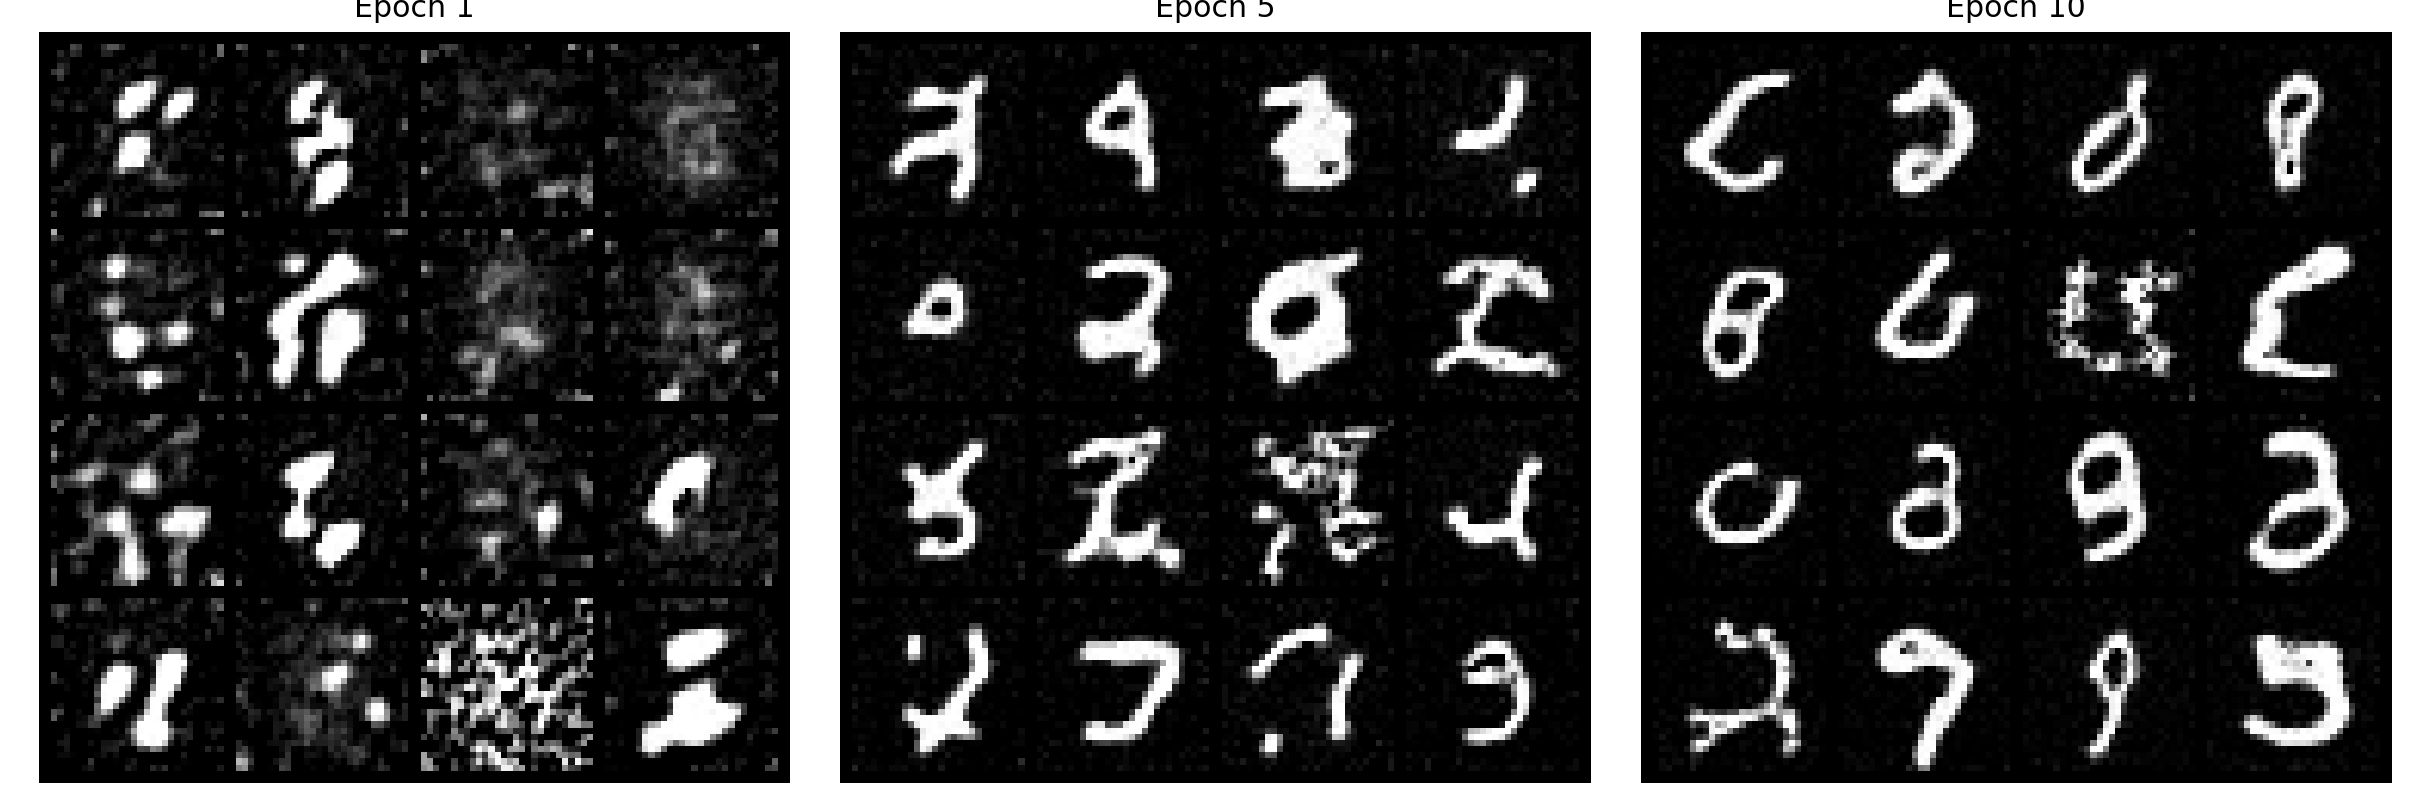
\includegraphics[width=0.95\linewidth]{../images/report/ebm_progress.png}
    \caption{Evolution of generated samples across training.}
    \label{fig:ebm-progress}
\end{figure}

\paragraph{First paragraph of analysis.}
At the beginning of training (left column) the generated images are
amorphous blobs that barely resemble digits.  The network has not yet
learned an energy landscape that favours the manifold of handwritten digits,
so the gradients guiding Langevin dynamics are nearly random.  After five
epochs (middle column) the shapes begin to coalesce into digit–like forms.
The sampler produces strokes and closed loops that hint at numbers such as
``3,'' ``8,'' and ``9.''  Some samples are still smeared or ambiguous,
reflecting the model's limited ability to distinguish fine structures at
this stage.

\paragraph{Second paragraph of analysis.}
By the tenth epoch (right column) the generated images are clearly
recognisable digits.  Most samples exhibit correct topology: one can
distinguish between digits with loops (``0,'' ``6,'' ``9'') and those with
straight lines (``1,'' ``7'').  Nevertheless, the images remain somewhat
blurry compared to real MNIST digits.  This blurriness arises from two
sources: the finite length of the Langevin chain and the smoothness of the
energy function.  Increasing the number of sampling steps beyond 60 can
sharpen the outputs but at the cost of additional computation.  Another
avenue for improvement is to use a more expressive architecture or to add
a learned step–size schedule; these enhancements are explored in more
advanced EBMs.

\subsection{Denoising Experiments}

In addition to unconditional generation, the assignment requires
demonstrating the model's denoising capabilities.  Given a noisy input
$\mathbf{x}_{\text{noisy}} = \mathbf{x} + \sigma\,\boldsymbol{\epsilon}$, where
$\boldsymbol{\epsilon}\sim\mathcal{N}(\mathbf{0},\mathbf{I})$ and $\sigma$ is
the noise level, we initialise Langevin dynamics at $\mathbf{x}_{\text{noisy}}$
and run a few iterations (typically three to ten) with a smaller step
size.  The intuition is that the energy gradient will guide the noisy
image back towards the nearest low–energy region corresponding to a clean
digit.  Figure~\ref{fig:ebm-denoise} depicts the denoising results for
three noise levels: $\sigma=0.2$, $\sigma=0.4$, and $\sigma=0.6$.

\begin{figure}[H]
    \centering
    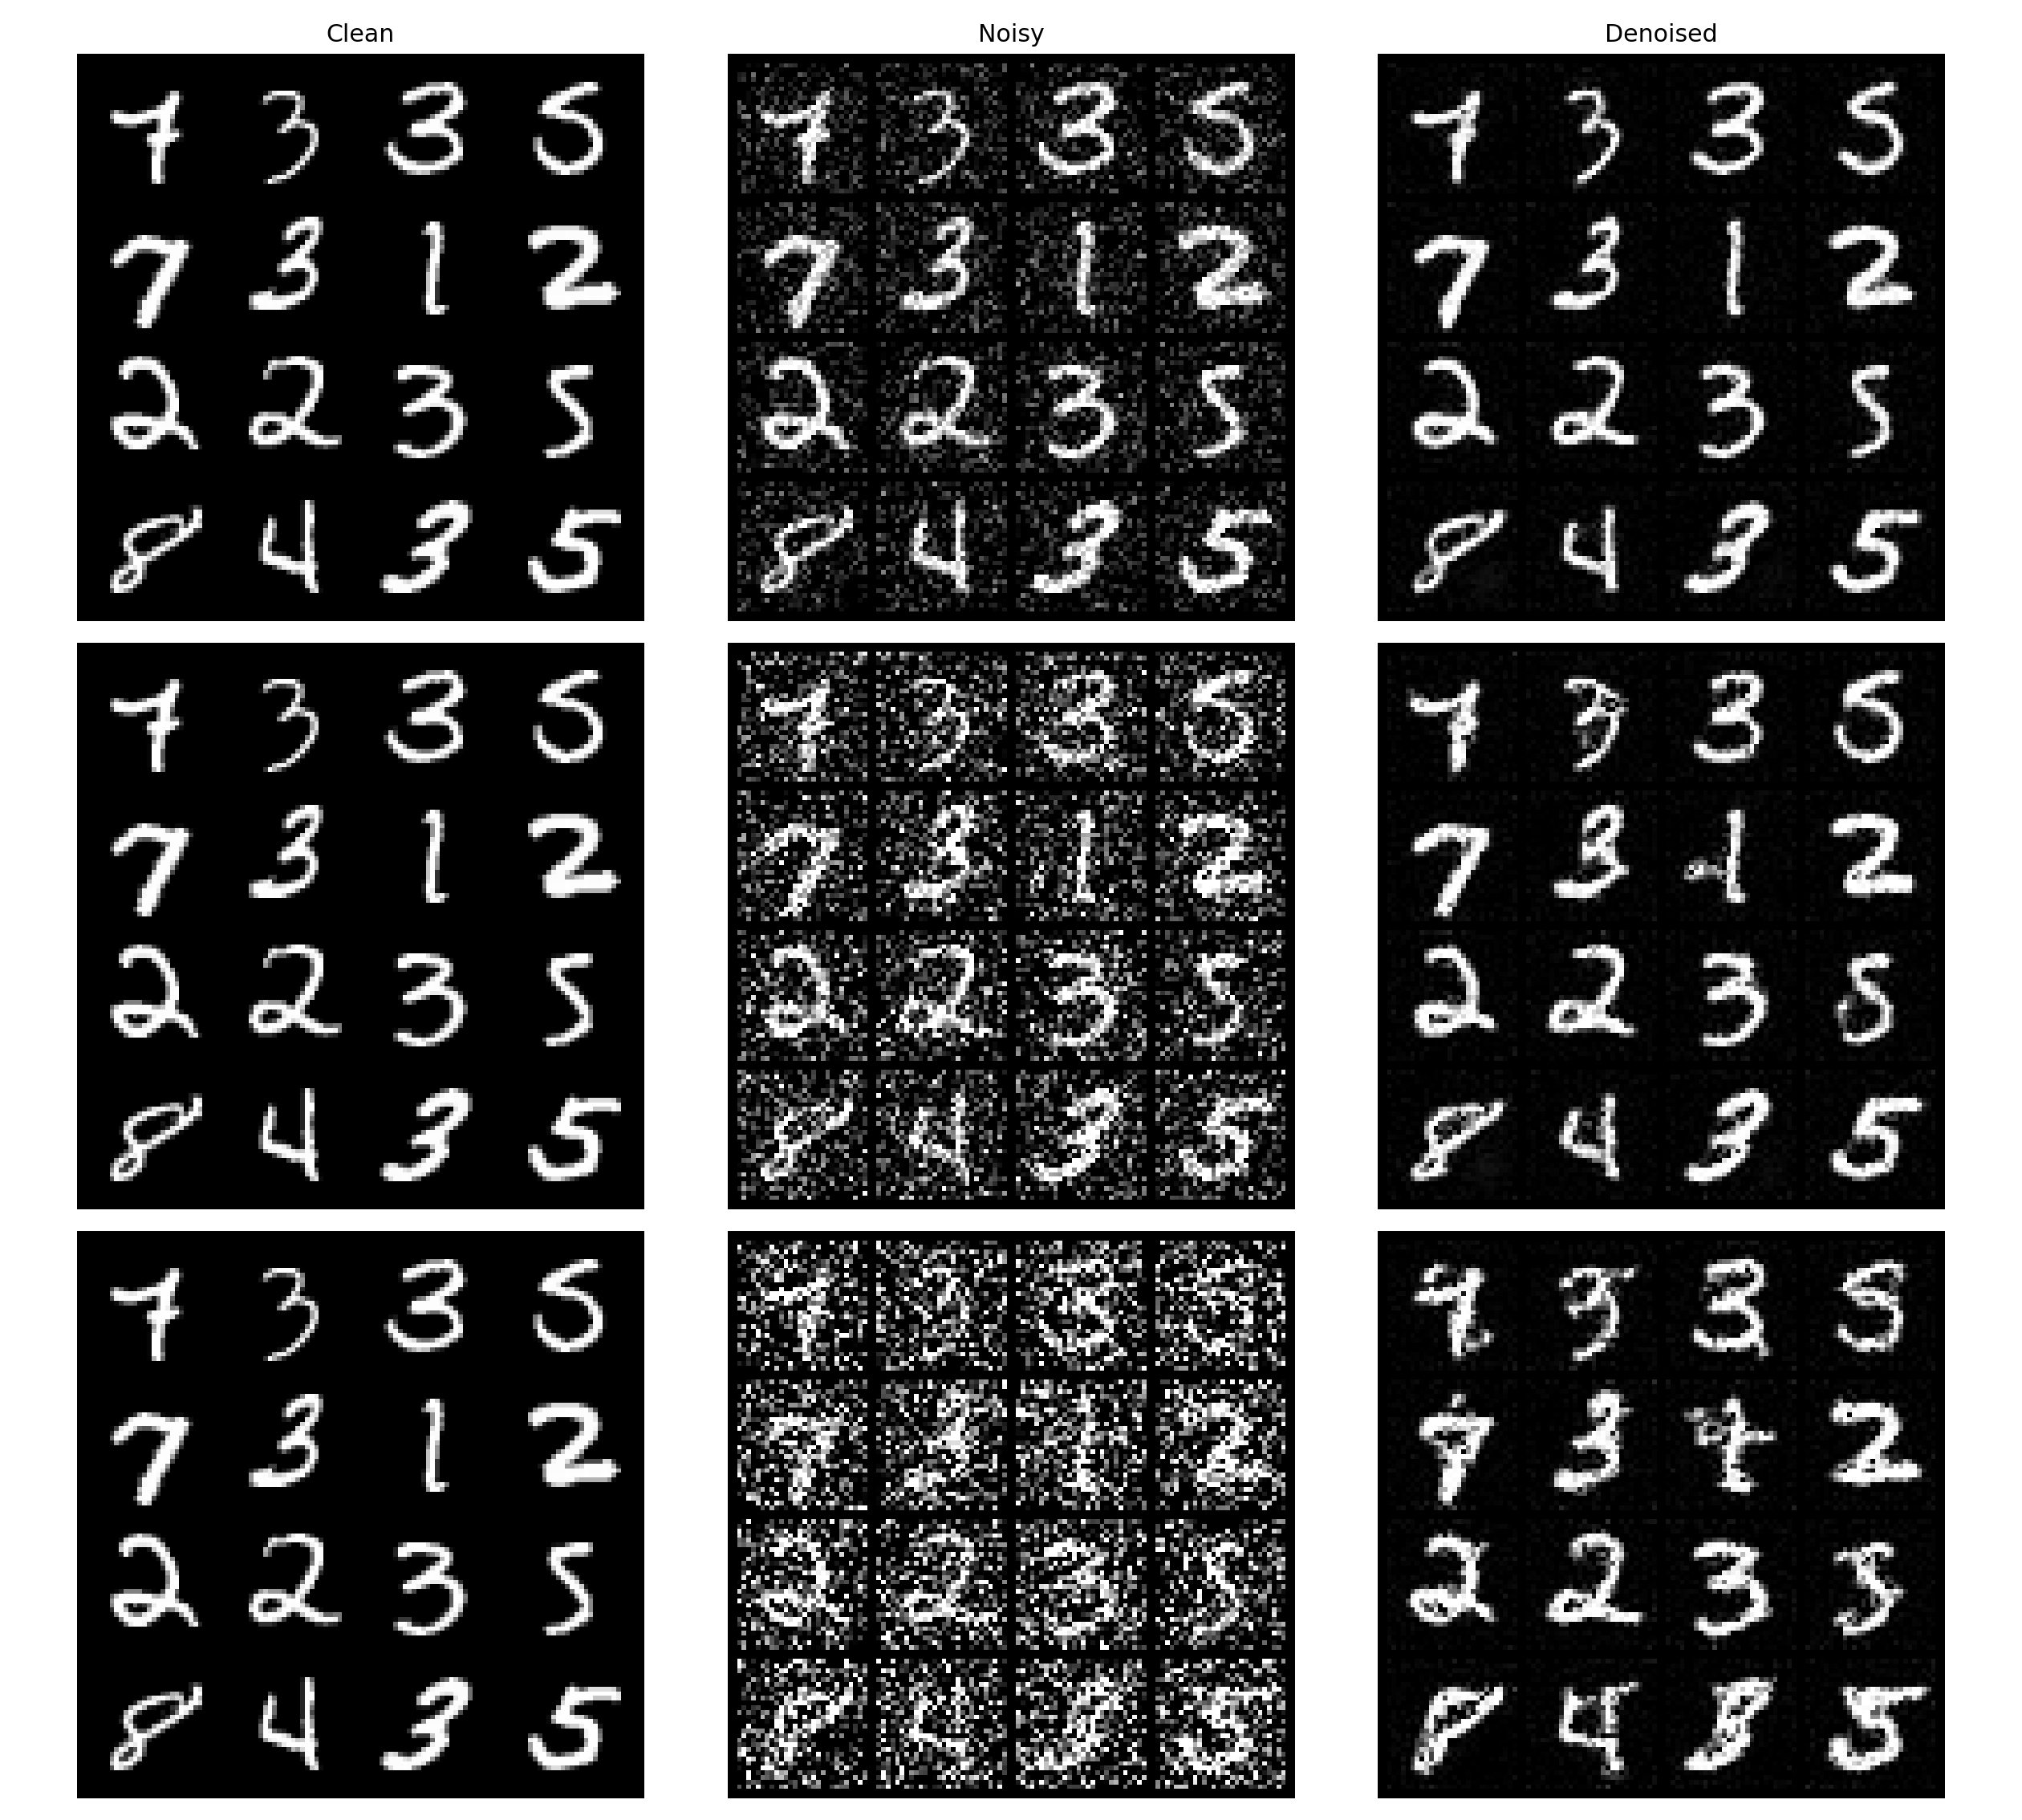
\includegraphics[width=0.95\linewidth]{../images/report/ebm_denoise.png}
    \caption{Denoising performance of the EBM at noise levels $\sigma=0.2$
    (top), $0.4$ (middle), and $0.6$ (bottom).}
    \label{fig:ebm-denoise}
\end{figure}

\paragraph{First paragraph of analysis (\texorpdfstring{$\sigma=0.2$}{sigma=0.2}).}
At a modest noise level of $0.2$, the noisy images still retain most of
their structural information.  The denoised outputs closely resemble the
original digits, with only minor blurring.  The model effectively removes
random speckles and small perturbations, especially along straight strokes
and within loops.  The energy landscape learned during training contains
smooth basins of attraction around each digit class, and Langevin dynamics
quickly guides the perturbed samples back into these basins.

\paragraph{Second paragraph of analysis (\texorpdfstring{$\sigma=0.4$}{sigma=0.4}).}
At a higher noise level of $0.4$, the digits become harder to recognise.
The denoising process still recovers the overall shape of many digits
(particularly ``1,'' ``7,'' and ``8''), but fine details are lost.  For
example, the tail of a ``2'' may blur into the loop of a ``6,'' and the
crossbar of a ``7'' may disappear.  In some cases the output looks like
the interpolation between two digit classes.  This behaviour reflects the
model's inability to perfectly reconstruct high–frequency details when the
initial perturbation is large.

\paragraph{Third paragraph of analysis (\texorpdfstring{$\sigma=0.6$}{sigma=0.6}).}
At an extreme noise level of $0.6$ the input images are nearly
indistinguishable from pure noise.  The denoised outputs still exhibit
digit–like patterns in some cases, but they are significantly blurred and
often mis–classified.  The model struggles to reconstruct complex
structures such as the crossing strokes of ``4'' or the open top of
``5.''  This failure is expected: the energy landscape was trained on
clean MNIST digits and does not contain sufficient curvature to recover
very noisy inputs.  Extending the Langevin chain helps only marginally,
and further improvements would require training with additional noise
regularisation or adopting score–based models designed for denoising.

\subsection{Refinement of Real Images}

An interesting application of EBMs is the refinement of real images.  By
running Langevin dynamics starting from a clean training example, the model
attempts to move the sample towards a lower–energy configuration.  We
selected a random batch of sixteen MNIST digits and applied 100 Langevin
steps with a small step size.  The refined images were almost identical
to the originals, with only slight sharpening of edges and suppression of
isolated noise pixels.  This observation suggests that the model has
learned an energy manifold that passes through the training data; the
gradient field does not dramatically distort examples already on the
manifold but nudges them towards canonical forms.  This behaviour contrasts
with that of score–based models, which we examine in Part~7.

\subsection{Hyperparameter Sensitivity and Limitations}

The quality of EBM samples is sensitive to several hyperparameters.  The
Langevin step size $\eta$ must be chosen carefully: too large a step
causes the chain to diverge or overshoot low–energy regions, producing
artefacts; too small a step slows mixing and leads to blurred samples.
Similarly, increasing the number of Langevin steps improves sample sharpness
but linearly increases computation.  We found that 60 steps with
$\eta=0.1$ strike a reasonable balance for MNIST.  The regularisation
coefficient $\lambda$ also plays a crucial role: lowering $\lambda$ to
$10^{-4}$ yields crisper images but occasionally leads to exploding
energies, whereas increasing $\lambda$ to $10^{-2}$ stabilises training at
the cost of excessive smoothing.  Finally, the replay buffer can reduce
gradient variance but may slow down adaptation if it contains stale
samples; a high replay ratio (e.g., $0.95$) was effective for MNIST but
would need tuning on larger datasets.

\subsection{Discussion of EBM Results}

Overall, the MNIST energy–based model captures the global structure of
handwritten digits and can generate recognisable samples after a few
epochs of training.  Its ability to denoise moderately perturbed images
demonstrates that the energy landscape contains meaningful basins around
the data manifold.  However, the model struggles with fine details,
especially when the noise level is high.  This limitation stems from the
local nature of the gradient–based sampler and the relatively simple
architecture.  In addition, training EBMs can be unstable; careful tuning
of the step size, number of steps, and regularisation is necessary.  The
subsequent parts of this report introduce score–based generative models,
which address many of these shortcomings by learning the score function
directly and employing a multi–scale noise schedule for sampling.
